%iffalse
\let\negmedspace\undefined
\let\negthickspace\undefined
\documentclass[journal,12pt,onecolumn]{IEEEtran}
\usepackage{cite}
\usepackage{amsmath,amssymb,amsfonts,amsthm}
\usepackage{algorithmic}
\usepackage{graphicx}
\usepackage{textcomp}
\usepackage{xcolor}
\usepackage{txfonts}
\usepackage{listings}
\usepackage{circuitikz}
\usepackage{enumitem}
\usepackage{tikz}
\usepackage{mathtools}
\usepackage{pgfplots}
\usepackage{gensymb}
\usepackage{comment}
\usepackage[breaklinks=true]{hyperref}
\usepackage{tkz-euclide} 
\usepackage{listings}
\usepackage{gvv}                                        
%\def\inputGnumericTable{}                                 
\usepackage[latin1]{inputenc}                                
\usepackage{color}                                            
\usepackage{array}                                            
\usepackage{longtable}                                       
\usepackage{calc}                                             
\usepackage{multirow}                                         
\usepackage{hhline}                                           
\usepackage{ifthen}                                           
\usepackage{lscape}
\usepackage{tabularx}
\usepackage{array}
\usepackage{float}

\usepackage{enumitem}
\usepackage{xcolor}
%\usepackage{multicol}


\newtheorem{theorem}{Theorem}[section]
\newtheorem{problem}{Problem}
\newtheorem{proposition}{Proposition}[section]
\newtheorem{lemma}{Lemma}[section]
\newtheorem{corollary}[theorem]{Corollary}
\newtheorem{example}{Example}[section]
\newtheorem{definition}[problem]{Definition}
\newcommand{\BEQA}{\begin{eqnarray}}
\newcommand{\EEQA}{\end{eqnarray}}
\newcommand{\define}{\stackrel{\triangle}{=}}
\theoremstyle{remark}
\newtheorem{rem}{Remark}

\title{2021-ST-1-13}
\author{AI24BTECH11023 - Tarun Reddy Pakala}
\begin{document}
\bibliographystyle{IEEEtran}

\maketitle
\bigskip
\renewcommand{\thefigure}{\theenumi}
\renewcommand{\thetable}{\theenumi}
\begin{enumerate}
\item The current population of a city is $11,02,500$. If it has been increasing at the rate of $5\%$ per annum, what was its population $2$ years ago ?
\begin{enumerate}
    \item $9,92,500$
    \item $9,95,006$
    \item $10,00,000$
    \item $12,51,506$
\end{enumerate}
\item $p$ and $q$ are positive integers and $\frac{p}{q}+\frac{q}{p}=3$, then, $\frac{p^2}{q^2}+\frac{q^2}{p^2}=$
\begin{enumerate}
    \item $3$
    \item $7$
    \item $9$
    \item $11$
\end{enumerate}
\item The least number of squares that must be added so that the line P-Q becomes the lines of symmetry is \underline{\hspace{2cm}}.
%input for figure 1
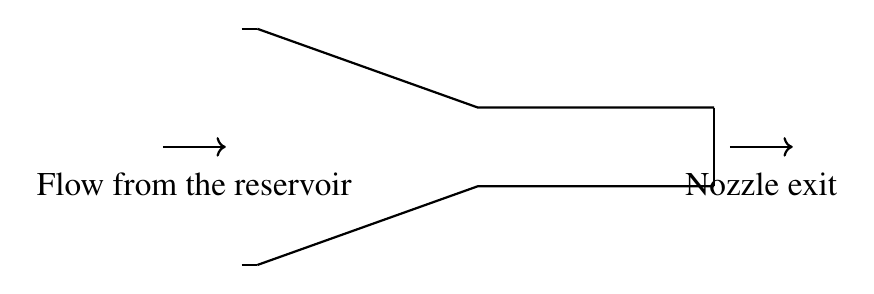
\begin{tikzpicture}
    % Draw the nozzle shape with short vertical lines at the opening
    \draw[thick] (-3,1.5) -- (-2.8,1.5);
    \draw[thick] (-3,-1.5) -- (-2.8,-1.5);
    \draw[thick] (-2.8,1.5) -- (0,0.5) -- (3,0.5);
    \draw[thick] (-2.8,-1.5) -- (0,-0.5) -- (3,-0.5);
    
    % Vertical line at the nozzle exit
    \draw[thick] (3,0.5) -- (3,-0.5);

    % Flow direction arrows
    \draw[->, thick] (-4,0) -- (-3.2,0);
    \draw[->, thick] (3.2,0) -- (4,0);

    % Labels for the flow and nozzle exit, placed below arrows
    \node[below] at (-3.6,-0.2) {\large Flow from the reservoir};
    \node[below] at (3.6,-0.2) {\large Nozzle exit};
\end{tikzpicture}

\begin{enumerate}
    \item $4$
    \item $3$
    \item $6$
    \item $7$
\end{enumerate}
\item $Nostalgia$ is to $anticipation$ as \underline{\hspace{2cm}} is to \underline{\hspace{2cm}}\\ Which one of the following options maintains a similar logical relation in the above sentence?
\begin{enumerate}
    \item Present,past 
    \item Future, past
    \item Past, future
    \item Future, present
\end{enumerate}
\item Consider the following sentences:\\
\brak{\textbf{i}} \; I woke up from sleep.\\
\brak{\textbf{ii}} \; I woked up from sleep.\\
\brak{\textbf{iii}} \;I was woken up from sleep.\\
\brak{\textbf{iv}} \;I was wokened up from sleep.\\
Which of the above sentences are grammatically CORRECT?
\begin{enumerate}
    \item \brak{\textbf{i}} and \brak{\textbf{ii}}
    \item \brak{\textbf{i}} and \brak{\textbf{iii}}
    \item \brak{\textbf{ii}} and \brak{\textbf{iii}}
    \item \brak{\textbf{i}} and \brak{\textbf{iv}}
\end{enumerate}
\subsection*{\textbf{Q.6-Q.10 Multiple Choice Questions (MCQ), carry two marks each (for each wrong answer: \(-\frac{2}{3}\))}}
\item Given below are two statements and two conclusions.\\
 Statement 1: \;All purple are green.\\
 Statement 2: \;All black are green.\\
 Conclusion I: \;Some black are purple.\\
 Conclusion II: \;No black is purple.\\
 Based on the above statements and conclusions, which one of the following options are logically CORRECT?
\begin{enumerate}
    \item Only conclusion I is correct.
    \item Only conclusion II is correct.
    \item Either conclusion I or II is correct.
    \item Both conclusion I and II are correct.
\end{enumerate}
\item Computers are ubiquitous. They are used to improve efficiency in almost all fields from agriculture to space exploration. Artificial intelligence \brak{AI} is currently a hot topic. AI enables computers to learn, give enough training data. For humans, sitting in front of computer for long hours can lead to health issues.\\ Which of the following can be deduced from the above passage?\\
\brak{i}\;Nowadays, computers are present in almost all places.\\
\brak{ii}\;Computers cannot be used for solving problems in engineering.\\
\brak{iii}\;For humans, there are both positive and negative effects of using computers.\\
\brak{iv}\;Artificial intelligence can be done without the data.
\begin{enumerate}
    \item \brak{ii} and \brak{iii}
    \item \brak{ii} and \brak{iv}
    \item \brak{i}, \brak{iii} and \brak{iv}
    \item \brak{i} and \brak{iii}
\end{enumerate}
\item Consider a square sheet of side $1$ unit. In the first step, it is cut along the main diagonal to get two triangles. In the next step, one of the cut triangles is revolved about its short edge to form a solid cone. The volume of the resulting cone, in cubic units, is \underline{\hspace{2cm}}.
\begin{enumerate}
    \item $\frac{\pi}{3}$
    \item $\frac{2\pi}{3}$
    \item $\frac{3\pi}{2}$
    \item $3\pi$
\end{enumerate}
\item 
%input for figure 2
\begin{figure}[!ht]
\centering
\resizebox{3cm}{3cm}{%
\begin{circuitikz}
\tikzstyle{every node}=[font=\LARGE]
\draw [ line width=0.6pt](2.75,12) to[sinusoidal voltage source, sources/symbol/rotate=auto] (3.25,11.5);
\draw [ line width=0.6pt](3.25,11.75) to[european resistor] (9.5,11.75);
\draw [line width=0.6pt, ->, >=Stealth] (9.5,11.75) -- (9.5,11);
\draw [ line width=0.6pt](4,12.25) to[short] (4,11.25);
\draw [ line width=0.6pt](4,11.5) to[short] (4,11);
\draw [ line width=0.6pt](8.75,12.25) to[short] (8.75,11);
\draw [ line width=0.6pt](4,11.25) to[short] (4.5,11.25);
\draw [ line width=0.6pt](8.75,11.25) to[short] (8.25,11.25);
\draw [ line width=0.6pt](4.25,11.25) to[short] (5.25,11.25);
\draw [ line width=0.6pt](8.25,11.25) to[short] (7.25,11.25);
\draw [ line width=0.6pt](5,11.25) to[european resistor] (5,8.5);
\draw [ line width=0.6pt](7.5,11.25) to[european resistor] (7.5,8.5);
\draw [ line width=0.6pt](4.75,8.5) to[short] (8,8.5);
\draw [line width=0.6pt, ->, >=Stealth] (6.25,8.5) -- (6.25,7.75);
\node [font=\normalsize] at (6.75,8) {Bus 3};
\node [font=\normalsize] at (4,12.5) {Bus 1};
\node [font=\normalsize] at (8.75,12.5) {Bus 2};
\node [font=\normalsize] at (6.25,12.25) {j q};
\node [font=\normalsize] at (4.5,10) {j r};
\node [font=\normalsize] at (8.25,9.75) {j p};
\end{circuitikz}
}%

\label{fig:my_label}
\end{figure}

The number of minutes spent by two students, \textbf{X} and \textbf{Y}, exercising every day in a given week are shown in the bar chart above.\\ The number of days in the given week in which one of the students spent a minimum $10\%$ more than the other student, on a given day, is
\begin{enumerate}
    \item $4$
    \item $5$
    \item $6$
    \item $7$
\end{enumerate}
\item 
Corners are cut from an equilateral triangle to produce a regular convex hexagon as shown in the figure above.\\ 
%input for figure 3
\begin{figure}[!ht]
\centering
\resizebox{3cm}{3cm}{%
\begin{circuitikz}
\tikzstyle{every node}=[font=\small]
\draw (4.25,12.25) to[battery1] (4.25,7.75);
\draw (4.25,12.25) to[short] (6.25,12.25);
\draw (4.25,7.75) to[short] (6.25,7.75);
\draw (6.25,12.25) to[R] (6.25,10.25);
\draw (6.25,10.25) to[R] (6.25,7.75);
\draw (6.25,10.25) to[short] (8.75,10.25);
\draw (6.25,7.75) to[short] (8.75,7.75);
\draw (8.75,7.75) to[R] (8.75,9.25);
\draw (8.75,10.25) to[D] (8.75,9);
\node [font=\small] at (4,10.25) {+};
\node [font=\small] at (4,9.75) {-};
\node [font=\small] at (4.75,10.5) {24 Volt};
\node [font=\small] at (6.75,11.25) {12 k$\Omega$};
\node [font=\small] at (6.75,9) {6 k$\Omega$};
\node [font=\small] at (8,8.5) {3.3 k$\Omega$};
\end{circuitikz}
}%

\label{fig:my_label}
\end{figure}

The ratio of the area of the regular convex hexagon to the area of the original equilateral triangle is
\begin{enumerate}
    \item $2\;:\;3$
    \item $3\;:\;4$
    \item $4\;:\;5$
    \item $5\;:\;6$
\end{enumerate}
\item Let $X$ be a non-constant positive random variable such that $E\brak{X}=9$. Then which one of the following statements is true?
\begin{enumerate}
    \item $E\brak{\frac{1}{X+1}}>0.1 \; \text{and} \; P\brak{X\geq10}\leq0.9$
    \item $E\brak{\frac{1}{X+1}}<0.1 \; \text{and} \; P\brak{X\geq10}\leq0.9$
    \item $E\brak{\frac{1}{X+1}}>0.1 \; \text{and} \; P\brak{X\geq10}>0.9$
    \item $E\brak{\frac{1}{X+1}}<0.1 \; \text{and} \; P\brak{X\geq10}>0.9$
\end{enumerate}
\item Let $\{W\brak{t}\}_{t\geq 0}$ be a standard Brownian motion. Then the variance of $W\brak{1}W\brak{2}$ equals
\begin{enumerate}
    \item $1$
    \item $2$
    \item $3$
    \item $4$
\end{enumerate}
\item Let $X_1,X_2,\ldots,X_n$ be a random sample of size n\brak{\geq 2} from a distribution having the probability density function
$$
f(x,\theta) = 
\begin{cases} 
    \frac{1}{\theta}e^{-\frac{x-\theta}{\theta}}, &  x > \theta \\ 
    0, &  otherwise 
\end{cases}
$$ where $\theta \in \brak{0,\infty}$. Then the method of moments estimator of $\theta$ equals
\begin{enumerate}
    \item $\frac{1}{2n}\sum_{i=1}^nX_i$
    \item $\frac{2}{n}\sum_{i=1}^nX_i$
    \item $\frac{1}{n}\sum_{i=1}^nX_i$
    \item $\frac{n}{\sum_{i=1}^{n}X_i}$
\end{enumerate}


\end{enumerate}
\end{document}
